\documentclass[../../main.tex]{subfiles}
\begin{document}

\begin{flushright}
\footnotesize\textit{【自動文字起こし・要確認】}
\end{flushright}

{\bf [解]}
円$O_k\ (k=1,2,\cdots,5)$の半径を$r_k$とすると，題意から
\begin{align}
r_1=1, \qquad r_2=a, \qquad r_3=r_4=\dfrac{1-a}{2}
\end{align}
である．又，$\angle DAB=\theta$とおく（$0<\theta<\pi/2\ \cdots$①）．

\begin{figure}[htb]
\begin{center}
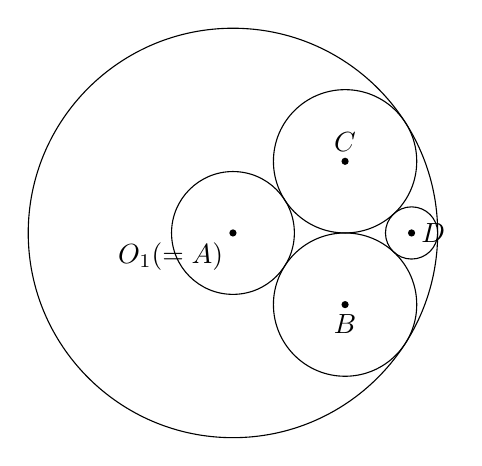
\begin{tikzpicture}[scale=1.3, >=stealth]
  % a=0.3 として図示 (円の半径は2倍に拡大: r1=2, r2=2a=0.6, r3=r4=2(1-a)/2=0.7, r5=2*0.1275)
  % O_1,O_2 は同心円 (中心は原点=A)
  \draw (0,0) circle (2);
  \draw (0,0) circle (0.6);
  \draw (1.0954,-0.7) circle (0.7);
  \draw (1.0954,0.7) circle (0.7);
  \draw (1.745,0) circle (0.255);
  \fill (0,0) circle (1pt) node[below left] {$O_1(=A)$};
  \fill (1.0954,0.7) circle (1pt) node[above] {$C$};
  \fill (1.0954,-0.7) circle (1pt) node[below] {$B$};
  \fill (1.745,0) circle (1pt) node[right] {$D$};
\end{tikzpicture}
\end{center}
\caption{円$O_1\sim O_5$の配置}
\end{figure}

$O_3$と$O_4$の接点を$E$とする．$E$は$AD$，$BC$の交点であることに注意する．

\textbf{(1)} ピタゴラスの定理から
\begin{align}
\begin{split}
AE&=\sqrt{\left(a+\dfrac{1-a}{2}\right)^2-\left(\dfrac{1-a}{2}\right)^2}=\sqrt{a} \quad\cdots * \\
DE&=\sqrt{\left(r_5+\dfrac{1-a}{2}\right)^2-\left(\dfrac{1-a}{2}\right)^2}=\sqrt{r_5^2+(1-a)r_5}
\end{split}
\end{align}
したがって，$r_1=1$を2通りで表して
\begin{align}
\begin{split}
1&=AE+DE+r_5=\sqrt{a}+\sqrt{r_5^2+(1-a)r_5}+r_5 \\
(1-\sqrt{a})-r_5&=\sqrt{r_5^2+(1-a)r_5} \\
r_5^2-2(1-\sqrt{a})r_5+(1-\sqrt{a})^2&=r_5^2+(1-a)r_5 \quad\cdots\text{②}, \qquad (1-\sqrt{a})-r_5\ge0\quad\cdots\text{③}
\end{split}
\end{align}
②から
\begin{align}
r_5=\dfrac{(1-\sqrt{a})^2}{2(1-\sqrt{a})+(1-a)}=\dfrac{(1-\sqrt{a})^2}{3-a-2\sqrt{a}}
\end{align}
である．$t=\sqrt{a}\ (0<t<1,\ \cdots$④$)$とおいて③に代入
\begin{align}
(1-t)+\dfrac{(1-t)^2}{t^2+2t-3}=(1-t)-\dfrac{1-t}{t+3}=\dfrac{(1-t)(t+2)}{t+3}\ge0\quad(\because④)
\end{align}
から，この$t$は③をみたして良い．この時，$*$から
\begin{align}
\begin{split}
DE&=\sqrt{\dfrac{1-t}{t+3}\left(\dfrac{1-t}{t+3}+1-t\right)}=\sqrt{\dfrac{(1-t)^2}{(t+3)^2}(t+2)^2}=\dfrac{(1-t)(t+2)}{t+3}\quad(\because④) \\
AE&=t
\end{split}
\end{align}
だから
\begin{align}
\begin{split}
S(a)&=\triangle ABD+\triangle ACD=AD\cdot BE=\left(t+\dfrac{(1-t)(t+2)}{t+3}\right)\cdot\dfrac{1-t^2}{2} \\
&=\dfrac{(t+1)(1-t)}{t+3}\cdot\dfrac{(\sqrt{a}+1)(1-\sqrt{a})}{\sqrt{a}+3}
\end{split}
\end{align}

\textbf{(2)} $f(t)=\dfrac{(t+1)(1-t)^2}{t+3}$とおく．$f(t)$の$0<t<1$での最大値をもとめれば良い．

$p=t+3$とおくと，$3<p<4$で，
\begin{align}
\begin{split}
f(t)&=\dfrac{(p-2)^2(4-p)}{p} \\
\dfrac{df}{dp}&=\dfrac{p[2(p-2)(4-p)-(p-2)^2]-(p-2)^2(4-p)}{p^2}=\dfrac{-2(p-2)(p^2-2p-4)}{p^2}
\end{split}
\end{align}
より，下表をうる．
\begin{center}
\begin{tabular}{c|ccccc}
$p$ & $3$ & & $1+\sqrt{5}$ & & $4$ \\
\hline
$f'$ & & $+$ & $0$ & $-$ & \\
\hline
$f$ & & $\nearrow$ & & $\searrow$ &
\end{tabular}
\end{center}
したがって，$p=1+\sqrt{5}$で最大値$10\sqrt{5}-22$をとる．


\newpage

\end{document}
